\chapter{Results}\label{cap:4}


{\lettrine[loversize=0.25,findent=0.2em,nindent=0em]{I}{n} this chapter, some examples of dynamic systems are used to compare the efficiency of the previously described algorithms. First, from the original system a discrete sequence \textit{S} over the alphabet $\Sigma$ of length \textit{N}$=10^7$ is generated. The frequencies of subsequences occurring in \textit{S} up to a length \textit{L}$_{max}$. After this, three PFSA are created using the D-Markov Machine, CRISSiS and our algorihm with different values of D, L and $L_1$ and $L_2$. Sequences of length \textit{N} are generated from each of those PFSA and using the metrics explained in Section \ref{sec:metrics} their performances are estimated. The results comparing the performances of the three algorithms' PFSA are then shown in Section \ref{sec:testcases}.

\section{Evaluation Metrics}\label{sec:metrics}

\subsection{Number of States}

This is the simplest comparison parameter. Each PFSA generated by the algorithms will have a set of states \textit{Q} of size |\textit{Q}|. When the original PFSA is known, it is useful to compare if the generated PFSA has a number of states close to the original. When that is not the case and all that is known is the original sequence, ideally it would be better to have a smaller PFSA to model the system. But there might be a trade-off where the smaller PFSA will result in the other metrics described in the following sections are deteriorated, while a bigger and more complex model achieves better performance. But given similar performances, the best model is the one with less states.

\subsection{Entropy Rate}

In Information Theory, entropy is a measure of the average information contained in a system. Using the definition in \cite{cover2012elements} and \citep{asok.14}, the Conditional Entropy is given by:

\begin{equation}
H(X|Y) \triangleq -\sum_{x\in X}P(x|Y)\log P(x|Y) . \label{eq:condent}
\end{equation}

The Entropy Rate is a measure of how dependent the current symbol of a sequence is on all the symbols that came before it and it is defined as:

\begin{equation}
h \triangleq \lim_{n\rightarrow\infty}H(X_n|X_1X_2\ldots X_{n-1}) = -\sum_{x\in X}P(x_n|X_1X_2\ldots X_{n-1})\log P(x_n|X_1X_2\ldots X_{n-1})  \label{eq:entrate}
\end{equation}

\noindent where $x_n$ is the n-th output symbol in the sequence \textit{S}. When Equation \ref{eq:entrate} converges for a certain \textit{n}, this indicates that the system that generated the sequence has a memory of \textit{n}, that is, knowing the \textit{n} previous symbols is enough to estimate the next one.

As it is not possible to compute Equation \ref{eq:entrate} up to infinity, we use the $\ell$-order Entropy Rate defined as:

\begin{equation}
h_{\ell} \triangleq H(X_{\ell}|X_1X_2\ldots X_{\ell-1}),   \label{eq:entratel}
\end{equation}

\noindent where $\ell$ should be chosen around a value where the system converges so the memory can be correctly estimated. If the entropy rate does not converge, it should be chosen to be at an inflection point. Comparing the values of $\ell$-order entropy rate of the generated PFSA with the one from the original system is useful to test if the generated one correctly captures the system memory.

\subsection{Kullback-Leibler Divergence}\label{sec:kld}

The Kullback-Leibler Divergence is a method to compare the distance between two probability distributions \textit{P} and \textit{Q}. Its formula is given by:

\begin{equation}
D(P||Q) = \sum_{i}P(i)\log(\frac{P(i)}{Q(i)}).	\label{eq:kld}
\end{equation}

Although it is technically not a distance, as it does not obey the triangle inequality nor is necessarily commutative, the Kullback-Leibler Divergence is useful to give an idea of how similar two distributions are. The smaller it is, the closer they are.

For the purpose of comparing the algorithms, consider two PFSA K$_1$ = ($\Sigma, Q_1, \delta_1, \mathcal{V}_1$) and K$_2$ = ($\Sigma, Q_2, \delta_2, \mathcal{V}_2$) over a common alphabet $\Sigma$. $P_1(\Sigma^{\ell})$ and $P_2(\Sigma^{\ell})$ are the steady state probability vectors of generating sequences of length $\ell$ from PFSA K$_1$ and K$_2$ respectively. For a given $\ell$ we take the $\ell$-order Kullback-Leibler Divergence as: 

\begin{equation}
D_{\ell}(K_1||K_2) = \sum_{\sigma\in\Sigma^{\ell}}P_1(\sigma)\log(\frac{P_1(\sigma)}{P_2(\sigma)}).	\label{eq:kldl}
\end{equation}

Instead of comparing the PFSA directly, $D_{\ell}$ can be used to compare the probability distribution of sub-sequences of length $\ell$ of a sequence generated by K$_1$ and another generated by K$_2$. A small divergence will indicate that the sequence generated by the algorithm is statistically close to the original sequence, which shows that the PFSA is a good estimate for the original system.

\subsection{$\Phi$-Metric}

The $\Phi$-Metric was presented in \citep{asok.14} as a way to compare to different PFSA. Given two PFSA K$_1$ = ($\Sigma, Q_1, \delta_1, \mathcal{V}_1$) and K$_2$ = ($\Sigma, Q_2, \delta_2, \mathcal{V}_2$) over a common alphabet $\Sigma$ and  $P_1(\Sigma^{\ell})$ and $P_2(\Sigma^{\ell})$  defined as in Section \ref{sec:kld}. The $\Phi$-Metric is then defined as:

\begin{equation}
\Phi(K1, K2) \triangleq \lim_{n\rightarrow\infty} \sum_{j = 1}^n \frac{\Vert P_1(\Sigma^j)-P_2(\Sigma^j)\Vert_{\ell_1}}{2^{j + 1}},\label{eq:phi}
\end{equation}

\noindent where $\Vert\star\Vert_{\ell_1}$ indicates the sum of absolute values of the elements in the vector $\star$. As Equation \ref{eq:phi} puts more weight in shorter words, it can be truncated with a relatively small $\ell$ by the $\ell$-order $\Phi$-Metric:

\begin{equation}
\Phi_{\ell}(K1, K2) \triangleq \sum_{j = 1}^{\ell} \frac{\Vert P_1(\Sigma^j)-P_2(\Sigma^j)\Vert_{\ell_1}}{2^{j + 1}}.\label{eq:phil}
\end{equation}

As with the Kullback-Leibler Divergence, the $\Phi$-Metric can be applied to compare a PFSA and a sequence generated by a PFSA or two PFSA-generated sequences by using the distribution of sub-sequences of length $\ell$. A small $\Phi$ indicates that the PFSA are similar to each other. For the performance comparison, each PFSA generated by the algorithms is compared with the original sequence using Equation $\ref{eq:phil}$ and the smaller the result, the better the algorithm models the original system.

\section{Test Cases}\label{sec:testcases}

\subsection{Ternary Even Shift}

The Ternary Even Shift is a symbolic dynamic system with a ternary alphabet where there can be no odd-numbered succession of non-zero symbols between zeros. This means that there must be an even number of 1's or two's between 0's. This is represented by the graph shown in Figure \ref{fig:ternaryeven}. For this system, 0 is a synchronization word.

\begin{figure}
\centering
\begin {tikzpicture}[-latex ,auto ,node distance =2 cm and 2 cm ,on grid ,
semithick ,
state/.style ={ circle , draw = black , text=black , minimum width =1 cm}]
\node[state] (0)
{$0$};
\node[state] (1) [below left=of 0] {$1$};
\node[state] (2) [below right =of 0] {$2$};
\path (0) edge [loop above] node[above = 0.1 cm] {$0|0.5$} (0);
\path (0) edge [bend left = 15] node[below = 0.3 cm] {$1|0.25$} (1);
\path (0) edge [bend right = 15] node[below =0.3 cm] {$2|0.25$} (2);
\path (1) edge [bend left =15] node[above = 0.25 cm] {$1|1.0$} (0);
\path (2) edge [bend right =15] node[above =0.25 cm] {$2|1.0$} (0);
\end{tikzpicture}
\caption{The graph of a Ternary Even-Shift.\label{fig:ternaryeven}}
\end{figure}

The results of our algorithm are compared to D-Markov and CRISSiS in Table \ref{tab:ternaryeven}. Our algorithm used the Omega termination and handed the same results for any L greater than 2. D-Markov machines of D = 6 and 7 were used. CRISSiS was tested using $L_1 = L_2 = 1$. It is possible to see that in this case, both CRISSiS and our algorithm reconstruct the same PFSA (shown in Figure \ref{fig:ternaryevengen}) and are a good estimate to the original PFSA  while a large D-Markov machine of at least 169 states is needed to obtain approximately the same performance. Even though D = 6 and 7, these D-Markov machines do not have 64 and 128 states respectively because there are forbidden words in the original system, which results in some states being non-existent in the RTP. The original system had $h_{10} = 1.0013$, which is close to the value found by all the algorithms.

\begin{figure}
\centering
\begin {tikzpicture}[-latex ,auto ,node distance =2.7 cm and 2.7 cm ,on grid ,
semithick ,
state/.style ={ circle , draw = black , text=black , minimum width =1 cm}]
\node[state] (0)
{$0$};
\node[state] (01) [below left=of 0] {$01$};
\node[state] (02) [below right =of 0] {$02$};
\path (0) edge [loop above] node[above = 0.1 cm] {$0|0.5001$} (0);
\path (0) edge [bend left = 15] node[below = 0.3 cm] {$1|0.2499$} (01);
\path (0) edge [bend right = 15] node[below =0.3 cm] {$2|0.2500$} (02);
\path (01) edge [bend left =15] node[above = 0.25 cm] {$1|1.0$} (0);
\path (02) edge [bend right =15] node[above =0.25 cm] {$2|1.0$} (0);
\end{tikzpicture}
\caption{The graph of a Ternary Even-Shift generated by out algorithm and by CRISSiS.\label{fig:ternaryevengen}}
\end{figure}

\begin{table}
\centering
\begin{tabular}{|l|c|c|c|}
\hline
 & \multicolumn{2}{c|}{\textbf{D-Markov}} & \textbf{Algo/CRISSiS}\\
 \hline
D/L & 6 & 7 & 2 \\
\hline
\# of States & 169 & 339 & 3 \\ 
$h_{10}$ & 1.0084 & 1.0058 & 1.0058 \\
$D_{10}$ & $2.7\cdot10^{-3}$ & $4.16\cdot10^{-5}$ & $9.55\cdot10^{-5}$ \\
$\Phi_{10}$  & $2.1\cdot10^{-3}$ & $1.2\cdot10^{-3}$ & $2.3\cdot10^{-3}$ \\
 \hline
\end{tabular}
\caption{Results for Ternary Even Shift. \label{tab:ternaryeven}}
\end{table}

\subsection{Tri-Shift}

The Tri-Shift was previously discussed in Section \ref{sec:crissis} and its graph is shown in Figure \ref{fig:trishift}. It was shown that its synchronization word is 00. The comparative results are shown in Table \ref{tab:trishift}. Once again this is an example where our algorithm and CRISSiS are able to recover the three states from the original PFSA with a good estimate for the morphs as seen in Figure \ref{fig:rectrishift}. To obtain a similar performance with a D-Markov machine, 128 or 256 states might be needed. The original system presented has $h_{10} = 0.9005$, showing that our algorithm, CRISSiS and the 7-Markov Machine are able to capture the system's memory.


\begin{figure}
\centering
\begin {tikzpicture}[-latex ,auto ,node distance =2.7 cm and 2.7 cm ,on grid ,
semithick ,
state/.style ={ circle , draw = black , text=black , minimum width =1 cm}]
\node[state] (A)
{$00$};
\node[state] (B) [above right=of A] {$001$};
\node[state] (C) [below right =of B] {$0010$};
\path (A) edge [loop left] node[above = 0.35cm] {$0|0.50002$} (A);
\path (A) edge [bend left = 15] node[above =0.35 cm] {$1|0.49998$} (B);
\path (B) edge [bend left = 15] node[above =0.35 cm] {$0|0.80002$} (C);
\path (B) edge [bend left = 15] node[below =0.45 cm] {$1|0.19998$} (A);
\path (C) edge [loop right] node[above = 0.35 cm] {$1|0.30007$} (C);
\path (C) edge [bend left = 15] node[below =0.15 cm] {$0|0.69993$} (A);
\end{tikzpicture}
\caption{The Tri-Shift PFSA generated by our algorithm and by CRISSiS.\label{fig:trishiftgen}}
\end{figure}

\begin{table}
\centering
\begin{tabular}{|l|c|c|c|}
\hline
 & \multicolumn{2}{c|}{\textbf{D-Markov}} & \textbf{Algo/CRISSiS}\\
 \hline
D/L & 7 & 8 & 2 \\
\hline
\# of States & 128 & 256 & 3 \\ 
$h_{10}$ & 0.9016 & 0.9005 & 0.9001 \\
$D_{10}$ & $4.1\cdot10^{-3}$ & $1.65\cdot10^{-3}$ & $1.16\cdot10^{-3}$ \\
$\Phi_{10}$ & $2.1\cdot10^{-3}$ & $7.2\cdot10^{-4}$ & $8.2\cdot10^{-4}$ \\
 \hline
\end{tabular}
\caption{Results for the Tri-Shift. \label{tab:trishift}}
\end{table}

\subsection{A Six State PFSA}

Figure \ref{fig:sixstate} shows a PFSA with six states that elucidates the differences between our algorithm and CRISSiS. This system has 4 synchronization words: 00, 01, 10 and 1111. The comparative results between the algorithms is show in Table \ref{tab:sixstate}.

\begin{figure}
\centering
\begin {tikzpicture}[-latex ,auto ,node distance =2.7 cm and 2.7 cm ,on grid ,
semithick ,
state/.style ={ circle , draw = black , text=black , minimum width =1 cm}]
\node[state] (A)
{$A$};
\node[state] (B) [below left=of A] {$B$};
\node[state] (C) [below right =of A] {$C$};
\node[state] (D) [below =of B] {$D$};
\node[state] (E) [below =of C] {$E$};
\node[state] (F) [below right =of D] {$F$};
\path (A) edge [loop above] node[above = 0.15cm] {$0|0.9$} (A);
\path (A) edge node[right = 0.15 cm] {$1|0.1$} (C);
\path (C) edge node[right = 0.15 cm] {$1|1.0$} (E);
\path (E) edge node[right = 0.15 cm] {$1|1.0$} (F);
\path (F) edge node[left = 0.15 cm] {$1|1.0$} (D);
\path (D) edge node[left = 0.15 cm] {$0|1.0$} (B);
\path (B) edge node[left =0.15 cm] {$0|0.5$} (A);
\path (B) edge node[below =0.15 cm] {$1|0.5$} (C);
\end{tikzpicture}
\caption{A Six-State PFSA.\label{fig:sixstate}}
\end{figure}

In this example, CRISSiS using $L_1 = L_2 = 1$ is not able to recover the original machine . It creates a PFSA with 2 states (Figure \ref{fig:sixstatecrissis}) which generates sequences fairly different from the original, as after a small transient, it outputs sequences of just 1's. On the other hand, by using any L larger than 4, our algorithm is capable of reconstructing a good estimate to the original system, shown in Figure \ref{fig:sixstatealgo}. For a D-Markov Machine to perform similarly, it is necessary to use D = 3 or 4, obtaining a PFSA with 7 and 11 states respectively. Once again, some sequences do not occur, therefore the D-Markov Machine in those cases will not have $2^D$ states.

\begin{table}
\centering
\begin{tabular}{|l|c|c|c|c|}
\hline
 & \multicolumn{2}{c|}{\textbf{D-Markov}} & \textbf{Algo} & \textbf{CRISSiS}\\
 \hline
D/L/$L_1$ and $L_2$ & 3 & 4 & 4 & 1/1\\
\hline
\# of States & 7 & 11 & 6 & 2 \\ 
$h_{10}$ & 0.5341 & 0.3344 & 0.3344 & $1.4427\cdot 10^{-7}$ \\
$D_{10}$ & 1.1980 & $4.0499\cdot 10^{-6}$ & $5.6969\cdot10^{-5}$ &  43.6556\\
$\Phi_{10}$ & $2.0005\cdot 10^{-3}$ & $4.6072\cdot 10^{-4}$ & $9.3745\cdot10^{-4}$ & 2.6505\\
 \hline
\end{tabular}
\caption{Results for the Six-State PFSA. \label{tab:sixstate}}
\end{table}

The results for this system show a type of system where CRISSiS performs badly. Starting from a single synchronization word and as many states have equal morphs and their paths will only be different after 3 steps, $L_2$ needs to be at least 3 to be able to recover the original PFSA and as CRISSiS' complexity is exponential on $L_2$ this means a hindrance in performance. As our algorithm uses all synchronization words, there are multiple starting points and the graph minimization algorithm step by the end is useful to differentiate states that will have different follower sets. The original system has a $h_{10} = 0.3344$, showing that both the 4-Markov Machine and our algorithm are able to estimate the system memory correctly.

\begin{figure}
\centering
\begin {tikzpicture}[-latex ,auto ,node distance =2.7 cm and 2.7 cm ,on grid ,
semithick ,
state/.style ={ circle , draw = black , text=black , minimum width =1 cm}]
\node[state] (A)
{$00$};
\node[state] (B) [right=of A] {$001$};
\path (A) edge [loop left] node[left = 0.15cm] {$0|0.9001$} (A);
\path (A) edge node[above = 0.15 cm] {$1|0.0999$} (B);
\path (B) edge [loop right] node[right = 0.15 cm] {$1|1.0$} (B);
\end{tikzpicture}
\caption{The Recovered Six-State PFSA by CRISSiS with $L_1 = L_2 = 1$.\label{fig:sixstatecrissis}}
\end{figure}

\begin{figure}
\centering
\begin {tikzpicture}[-latex ,auto ,node distance =2.7 cm and 2.7 cm ,on grid ,
semithick ,
state/.style ={ circle , draw = black , text=black , minimum width =1 cm}]
\node[state] (A)
{$00$};
\node[state] (B) [below left=of A] {$10$};
\node[state] (C) [below right =of A] {$01$};
\node[state] (D) [below =of B] {$1111$};
\node[state] (E) [below =of C] {$011$};
\node[state] (F) [below right =of D] {$0111$};
\path (A) edge [loop above] node[above = 0.15cm] {$0|0.9001$} (A);
\path (A) edge node[right = 0.15 cm] {$1|0.0999$} (C);
\path (C) edge node[right = 0.15 cm] {$1|1.0$} (E);
\path (E) edge node[right = 0.15 cm] {$1|1.0$} (F);
\path (F) edge node[left = 0.15 cm] {$1|1.0$} (D);
\path (D) edge node[left = 0.15 cm] {$0|1.0$} (B);
\path (B) edge node[left =0.15 cm] {$0|0.5001$} (A);
\path (B) edge node[below =0.15 cm] {$1|0.4999$} (C);
\end{tikzpicture}
\caption{The Recovered Six-State PFSA by our algorithm.\label{fig:sixstatealgo}}
\end{figure}

\subsection{Maximum Entropy \textit{(d,k)}-Constrained Code}

As seen in \cite{immink.98}, a \textit{(d,k)}-constrained code is a code used in digital recording devices and other systems in which a long sequences of 1's might cause desynchronization issues. This code guarantees that at lest \textit{d} 1's are generated between occurrences of 0's and that after \textit{k} 1's, a 0 has to appear. A Maximum Entropy \textit{(d,k)}-Constrained Code is a PFSA that generates sequences with those restrictions and that also have maximum information entropy. The algorithms were tested to recover a Maximum Entropy (3,5)-Constrained Code shown in Figure \ref{fig:dk_35}. To achieve maximum entropy, a parameter $\lambda$ has to be set at 1.24985. The synchronization words for this system are 0 and 11111.

\begin{figure}
\centering
\begin {tikzpicture}[-latex ,auto ,node distance =2.7 cm and 2.7 cm ,on grid ,
semithick ,
state/.style ={ circle , draw = black , text=black , minimum width =1 cm}]
\node[state] (A)
{$A$};
\node[state] (B) [right =of A] {$B$};
\node[state] (C) [right =of B] {$C$};
\node[state] (D) [right =of C] {$D$};
\node[state] (E) [right =of D] {$E$};
\node[state] (F) [right =of E] {$F$};
\path (A) edge node[below = 0.15cm] {$1|1.0$} (B);
\path (B) edge node[below = 0.15 cm] {$1|1.0$} (C);
\path (C) edge node[below = 0.15 cm] {$1|1.0$} (D);
\path (D) edge node[below = 0.15 cm] {$1|0.5902$} (E);
\path (D) edge [bend right] node[below = 0.15 cm] {$0|0.4908$} (A);
\path (E) edge node[below = 0.15 cm] {$1|0.4445$} (F);
\path (E) edge [bend right] node[right =1.75 cm] {$0|0.5555$} (A);
\path (F) edge [bend right] node[right =2.5 cm] {$0|1.0$} (A);
\end{tikzpicture}
\caption{The Maximum Entropy (3,5)-Constrained Code PFSA.\label{fig:dk_35}}
\end{figure}

The results for this system are shown in Table \ref{tab:dk35}. This is a practical case where CRISSiS needs a higher $L_2$ to obtain a correct estimate, implying a cubic complexity. When $L_2$ is 3, CRISSiS recovers the same PFSA as our algorithm (shown in Figure \ref{fig:dk_35r}) and perform equally well. On the other hand, when $L_2$ is lower than 3, CRISSiS creates a PFSA with one state that continually generates the symbol 1, which performs poorly. The original $h_{10}$ is 0.3218, showing that both CRISSiS and our algorithm are able to capture the system memory correctly. For a D-Markov Machine to have a similarly good performance, a D of 5 is needed, generating machines of 7 states, which are bigger than the original PFSA.

\begin{table}
\centering
\begin{tabular}{|l|c|c|c|c|c|}
\hline
 & \multicolumn{2}{c|}{\textbf{D-Markov}} & \textbf{Algo} & \multicolumn{2}{|c|}{\textbf{CRISSiS}}\\
 \hline
D/L/$L_1$ and $L_2$ & 4 & 5 & 6 & 1/1 & 1/3\\
\hline
\# of States & 5 & 7 & 6 & 1 & 6\\ 
$h_{10}$ & 0.3575 & 0.3218 & 0.3218 & $1.4427\cdot 10^{-7}$ & 0.3218\\
$D_{10}$ & 0.1793 & $7.0139\cdot 10^{-7}$ &  $2.3766\dot 10^{-6}$ & 45.5434 & $5.9715\cdot 10^{-7}$\\
$\Phi_{10}$ & $5.0521\cdot 10^{-3}$ & $1.5380\cdot 10^{-4}$ & $2.8001\cdot 10^{-4}$ & 1.5165 & $9.3656\cdot 10^{-5}$ \\
 \hline
\end{tabular}
\caption{Results for the Maximum Entropy (3,5)-Constrained Code PFSA. \label{tab:dk35}}
\end{table}

\begin{figure}
\centering
\begin {tikzpicture}[-latex ,auto ,node distance =2.7 cm and 2.7 cm ,on grid ,
semithick ,
state/.style ={ circle , draw = black , text=black , minimum width =1 cm}]
\node[state] (A)
{$0$};
\node[state] (B) [right =of A] {$01$};
\node[state] (C) [right =of B] {$011$};
\node[state] (D) [right =of C] {$0111$};
\node[state] (E) [right =of D] {$01111$};
\node[state] (F) [right =of E] {$11111$};
\path (A) edge node[below = 0.15cm] {$1|1.0$} (B);
\path (B) edge node[below = 0.15 cm] {$1|1.0$} (C);
\path (C) edge node[below = 0.15 cm] {$1|1.0$} (D);
\path (D) edge node[below = 0.15 cm] {$1|0.5902$} (E);
\path (D) edge [bend right] node[below = 0.15 cm] {$0|0.4908$} (A);
\path (E) edge node[below = 0.15 cm] {$1|0.4437$} (F);
\path (E) edge [bend right] node[right =1.75 cm] {$0|0.5563$} (A);
\path (F) edge [bend right] node[right =2.5 cm] {$0|1.0$} (A);
\end{tikzpicture}
\caption{The Maximum Entropy (3,5)-Constrained Code PFSA recovered by our algoritum and by CRISSiS.\label{fig:dk_35r}}
\end{figure}

\subsection{Logistic Map}

The next two examples show how the algorithms fare when modeling a system whose PFSA is unknown or non-existent. A sequence from these systems will be analyzed and a PFSA model will be created and its output will be compared to the original sequence to see how well this Markovian model approximates a dynamic system which might not even be Markovian.

The first of these examples is the Logistic Map, a symbolic dynamic system whose outputs is given by the difference equation \cite{asok.14}:

\begin{equation}
x_{k+1} \triangleq rx_k(1-x_k), \label{eq:logisticmap}
\end{equation}


\noindent which shows chaotic behavior when the \textit{r} parameter is approximately 3.57. As in \cite{asok.14}, the initial x is set to 0.5 and \textit{r} = 3.75. A sequence of length $10^{-7}$ was generated from this equation and then it was quantized with a ternary alphabet: values x$_k \leq 0.67$ were mapped to 0; when 0.67 < x$_k \leq 0.79$, it was mapped to 1 and when x$_k$ > 0.79 it was mapped to 2. A part of that sequence and the specified threshold are shown in Figure \ref{fig:lmapseq}.

\begin{figure}
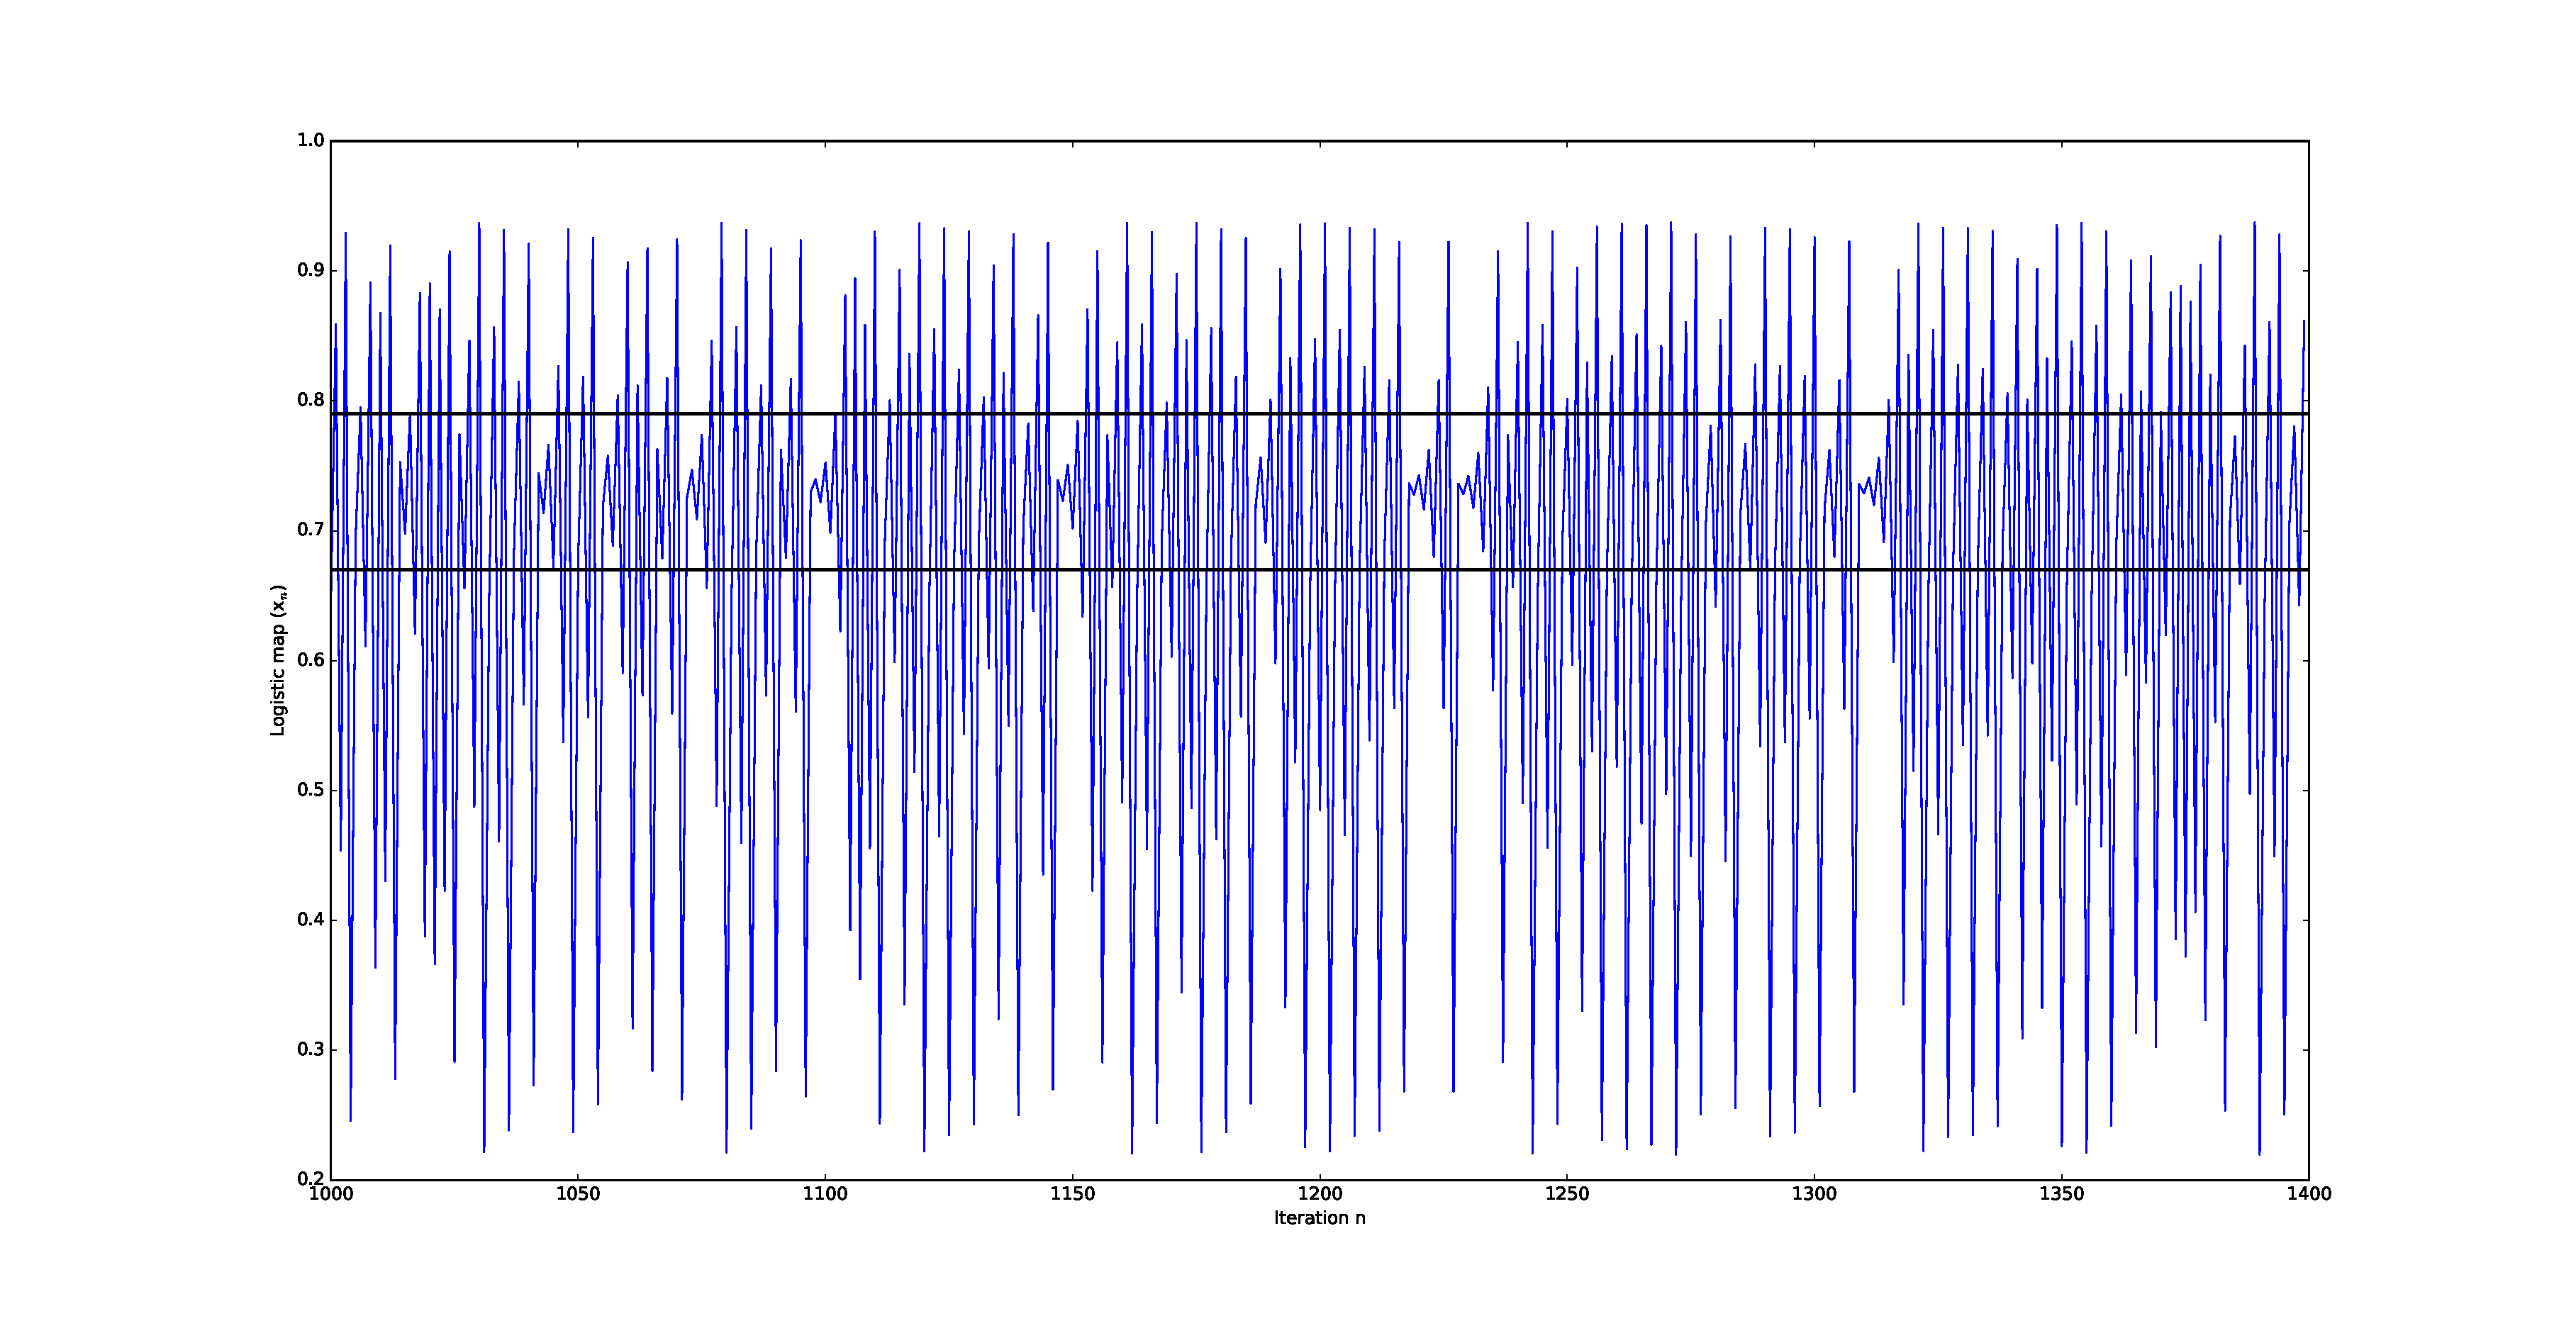
\includegraphics[scale=0.25]{Figuras/logisticmap.eps}
\caption{Part of the Logistic Map generated by Equation \ref{eq:logisticmap} with x$_0$ = 0.5 and $r$ = 3.75.\label{fig:lmapseq}}
\end{figure}

From this ternary sequence, the three algorithms were applied in order to obtain a Markovian model for the logistic map.

\subsection{Gilbert-Elliot Channel}

The Gilbert-Elliot Channel (GEC) is used to model digital communication channels that suffer with burst errors, i.e. a channel that usually has low probability of error but that has moments where many sequential errors occur. As described in \cite{mushkin.89}, Figure \ref{fig:gec} is the GEC model. It operates in two states, \textit{0} (the "good channel") and \textit{1} (the "bad channel"). While it is in \textit{0}, it works as a Binary Symmetric Channel (BSC) with error probability of $p_0$, which is usually very small, indicating a state in which the channel does not produce too many errors. When it is in state \textit{1}, it is a BSC with error probability $p_1$ which is higher than $p_0$, indicating a state where it is more probable for an error to occur. When in state \textit{0}, it has a probability $q$ of transitioning to state \textit{1} and $1-q$ to stay in \textit{0}. Similarly, when in \textit{1}, it transitions to \textit{0} with probability $q$ and stays with probability $1-q$. This indicates that there is a chance from going to one situation to the other.

\begin{figure}
\centering
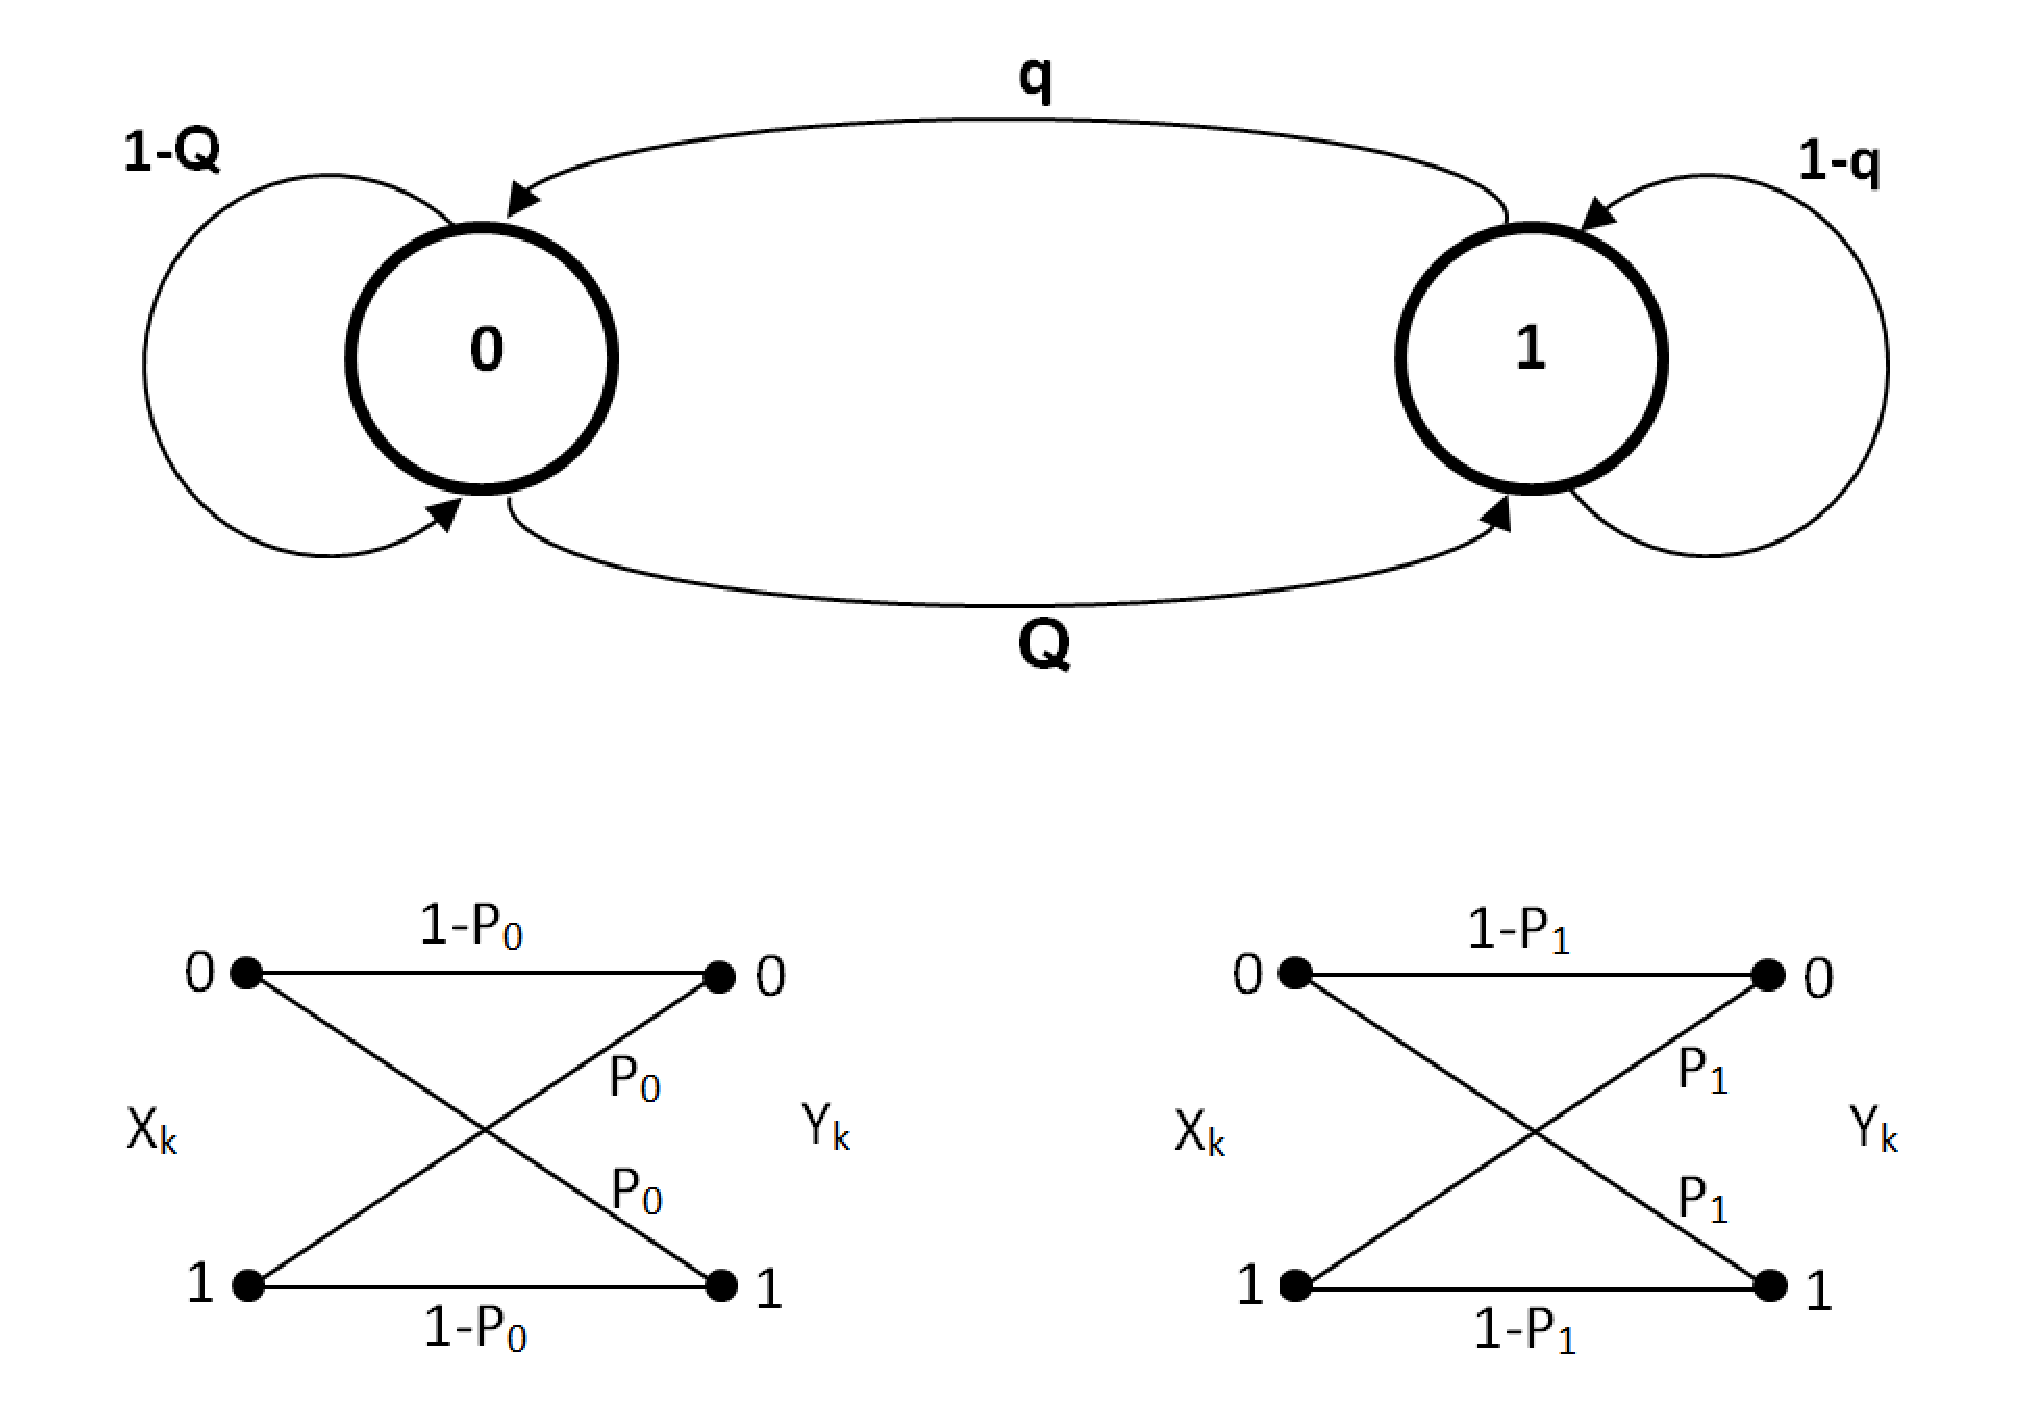
\includegraphics[width=8cm, height=6cm]{Figuras/figgec.eps}
\caption{\label{fig:gec} The Gilbert-Elliott Channel.}
\end{figure}

Other important parameters of the GEC that need to be evaluated are its memory $\mu$ and the Bit Error Rate (BER), which is a percentage of errors in the transmission. The memory $\mu$ is defined as:

\begin{equation}
\mu = 1 - q - Q. \label{eq:mumemory}
\end{equation}

\noindent which reduces to a memoryless BSC when $\mu = 0$. This parameter is called memory because, as seen in \cite{mushkin.89}, the GEC's autocorrelation function is:

\begin{equation}
R_{GEC}[m] = (\text{BER})^2 +\frac{Qq(p_1-p_0)²}{(q+Q)²}(1-q-Q)^m, \label{eq:rgec}
\end{equation}

\noindent which, without getting into much detail, shows that $\mu$ influences how a symbol is related to another one that is $m$ symbols apart. The BER is given by:

\begin{equation}
\text{BER} = \frac{q}{q+Q}p_0 + \frac{Q}{q+Q}p_1. \label{eq:gecber}
\end{equation}

The GEC can be designed to obtain specific values of $\mu$ and BER and then it is possible to compare how close to the design parameters the generated PFSA are able to get in order to evaluate their performance.

A binary sequence going through this channel would be output in instant $k$ the following way:

\begin{equation}
y_k = x_k\oplus z_k, \label{eq:binarychannel}
\end{equation}


\noindent in which $x_k$ is the input symbol at instant $k$, $z_k$ is the error symbol at instant $k$ and $\oplus$ is binary addition operation. When $z_k$ is 0, $y_k$ will be equal to $x_k$, which means that no error occurred. On the other hand, when it 1, $y_k$ will be $x_k \oplus 1 = \neg x_k$, indicating the occurrence of an error. The symbol $z_k$ has a probability $p_e$ of being 1 and $1-p_e$ of being 0 and $p_e$ is equal to $p_0$ if the channel is in state \textit{0} and equal to $p_1$ when it is in state \textit{1}. Following this rule, an error sequence $z$ can be generated to model how the channel and how it affects an input sequence. An error sequence of length $10^{7}$ is generated and used as input to the algorithms. The GEC is strictly not Markovian and this is an example to show how the algorithms fare in modeling such a system in a Markovian fashion.